%%%  \chapter{Writing Standard }

%%%%%%%%%%%%%%%%%%%%%%%%%%%%%%%%%%%%%%%%%%%%%%
\section{Some Instructions and Coding Standards}

A few notes:

It's helpful to add the lines of percents ahead of section delimiters for navigating through the tex document. (I have it so that it renders in color.)  Longer lines for sections, half as long for subsections, half again as long for subsubsections.

To compile the document, run pdflatex protodune-tdr

To update the Table of Contents, run that command twice.  To get everything run ./compileitdraft protodune-tdr.

The list of acronyms is copied from the CDR and will need reworking. It's controlled by some files under the common directory. We'll worry about it later!

%%%%%%%%%%%%%%%%%%%%%%%%%%
\subsection{fixme}
Here's how to add a ``fixme'':
\fixme{testing}
Fixmes and line numbers will show up when you compile as draft (use ./compileitdraft protodune-tdr).

They will not show up when you compile as print (use ./compileitprint protodune-tdr).

%%%%%%%%%%%%%%
\subsubsection{Here's a subsubsection}
...with some text.

You cannot have only one section in a chapter (because that implies that the chapter doesn't need subdivision), nor can you have only one subsection in a section (for the same reason).


%%%%%%%%%%%%%%%%%%%%%%%%%%
\subsection{Figures}
There's an enviroment defined as cdrfigure, and all you need to do for a figure in your file is fill in the following (as it appears in the tex file, not the pdf) with the short caption, the label (without ``fig:'' at the front), the long caption and then the filename with the appropriate width:

\begin{cdrfigure}[short caption for table of figures]{label}{long caption that appears below picture}
  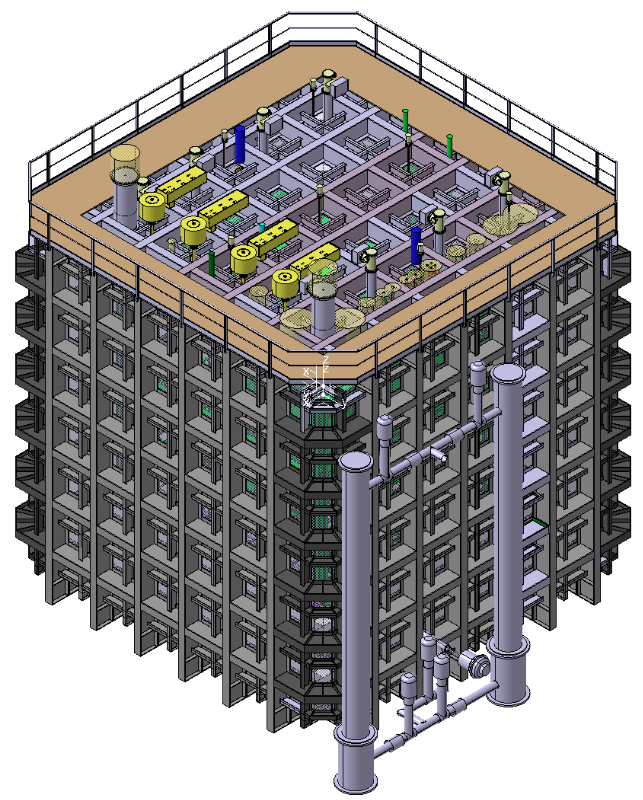
\includegraphics[width=0.8\textwidth]{protoDUNE_cryostat.png}
\end{cdrfigure}

The reference that points to it needs to read Figure~\ref{fig:label} (i.e., with the ``fig:'')


For tables, it's similar:

\begin{cdrtable}[short caption for table of tables]{cc}{label}{long caption to appear above table}
Header Column1 & Header Column 2 \\ \toprowrule
Row 1 & First \\ \colhline
Row 2 & Second \\ \colhline
Row 3 & Third \\
\end{cdrtable}

The third argument (reads {cc}) can use c, l, r, p{some length} but please do not include lines like `'|c|l|l|''.

The reference that points to it needs to read Table~\ref{tab:label} (i.e., with the ``tab:'')

%%%%%%%%%%%%%%%%%%%%%%%%%%
\subsection{References}

In the file common/pdune-tdr-citedb.bib there are a few citations listed as examples. Please follow the format shown.  To add a reference within the text, do it like this:  ``Blah blah blah. This is described further in~\cite{cdr-annex-singleph-proto}.''

The references are not compiled with a simple run of pdflatex, you have to run the bibtex command.  It's included in the scripts compileitdraft and compileitprint.


%%%%%%%%%%%%%%%%%%%%%%%%%%
\subsection{git reference}

Install git (see https://github.com/).
Clone repository (See ``Initial Clone'' in instructions at https://github.com/DUNE/document-guidance.)
General editing procedure

\begin{itemize}
\item    cd to directory into which you cloned document
\item  git pull
\item    (Edit files. Then test that document compiles.)
\item    pdflatex volume-x
\item    (Fix editing errors and retry until it compiles.)
\item    git pull (yes, again, for good measure)
\item    (If you have new files, add them.)
\item    git add volume-x/new-file.tex
\item    git add volume-x/figures/new-image-file.pdf
\item    git commit -a -m "some commit message"
\item    git push
\end{itemize}

If git pull fails:

\begin{itemize}
\item       git stash
\item      git pull
\item      git stash pop
\item      (Fix conflicts, commit and push.)
\end{itemize}

(Delete to here once you know how to do all this stuff.)

%%%%%%%%%%%%%%%%%%%%%%%%%%%%%%%%%%%%%%%%%%%%%%%%%%%%
\section{Next Section}

%%%%%%%%%%%%%%%%%%%%%%%%%%%%%%%%%%%%%%%%%%%%%%%%%%%%
\section{And the Next One}

%%%%%%%%%%%%%%%%%%%%%%%%%%
\subsection{Subsec 1}


%%%%%%%%%%%%%%%%%%%%%%%%%%
\subsection{Subsec 2}


